% =====================================================================
% BMED365: Neural Networks and Deep Learning
% Beamer presentation - Topic List D01-D13
% =====================================================================
\documentclass[aspectratio=169, 10pt]{beamer}

% =====================================================================
% PACKAGES
% =====================================================================
\usepackage[utf8]{inputenc}
\usepackage[T1]{fontenc}
\usepackage[english]{babel}
\usepackage{graphicx}
\usepackage{tikz}
\usetikzlibrary{shapes.geometric, arrows, positioning, calc, decorations.pathreplacing}
\usepackage{booktabs}
\usepackage{amsmath}
\usepackage{fontawesome5}

% =====================================================================
% THEME AND COLORS
% =====================================================================
\usetheme{Madrid}
\usecolortheme{beaver}

% Colors for TikZ diagrams
\definecolor{uibblue}{RGB}{0, 61, 115}
\definecolor{uibred}{RGB}{175, 28, 44}

% =====================================================================
% TITLE INFO
% =====================================================================
\title{Neural Networks and Deep Learning}
\subtitle{BMED365: Topic List D01--D13}
\author{BMED365}
\date{Spring 2026}

% =====================================================================
% DOCUMENT
% =====================================================================
\begin{document}

% Title page
\begin{frame}
    \titlepage
\end{frame}

% Table of Contents
\begin{frame}{Overview}
    \tableofcontents
\end{frame}

% =====================================================================
% SECTION: Biological vs. Artificial Neurons
% =====================================================================
\section{Basic Neural Networks}

\begin{frame}{D01: Compare biological and artificial neurons}
    \begin{columns}[T]
        \begin{column}{0.48\textwidth}
            \textbf{Biological neuron:}
            \begin{itemize}
                \item \textbf{Dendrites:} Receives signals
                \item \textbf{Cell body:} Processes
                \item \textbf{Axon:} Transmits
                \item \textbf{Synapse:} Connection to next neuron
                \item Complex electrochemical activity
            \end{itemize}
        \end{column}
        \begin{column}{0.48\textwidth}
            \textbf{Artificial neuron (perceptron):}
            \begin{itemize}
                \item \textbf{Inputs} $x_1, x_2, \ldots$: Receives data
                \item \textbf{Weights} $w_1, w_2, \ldots$: Synaptic strength
                \item \textbf{Sum:} $z = \sum w_i x_i + b$
                \item \textbf{Activation:} $a = f(z)$ \small(f = activation function)
                \item Mathematical simplification
            \end{itemize}
        \end{column}
    \end{columns}
    
    \vspace{0.5cm}
    \begin{block}{Key similarity}
        Both sum incoming signals and ``fire'' (activate) if total stimulation exceeds a threshold.
    \end{block}
    
    \begin{alertblock}{Important difference}
        Artificial neurons are \textbf{greatly simplified models} - they do not capture the full complexity of the brain.
    \end{alertblock}
\end{frame}

\begin{frame}{D02: Describe the structure of a multilayer perceptron (MLP)}
    \begin{columns}[T]
        \begin{column}{0.55\textwidth}
            \textbf{MLP architecture:}
            \begin{itemize}
                \item \textbf{Input layer:} Receives features (no processing)
                \item \textbf{Hidden layers:} One or more layers of neurons
                \item \textbf{Output layer:} Produces prediction
            \end{itemize}
            
            \vspace{0.3cm}
            \textbf{Fully connected (dense):}
            \begin{itemize}
                \item Each neuron in one layer is connected to \textbf{all} neurons in the next layer
                \item Many parameters (weights and biases)
            \end{itemize}
            
            \vspace{0.3cm}
            \textbf{``Deep'' learning:}
            \begin{itemize}
                \item $\geq$ 2 hidden layers = deep model
                \item More layers $\rightarrow$ more abstract representations
            \end{itemize}
        \end{column}
        \begin{column}{0.42\textwidth}
            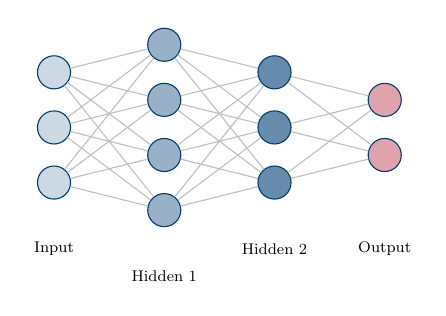
\begin{tikzpicture}[scale=0.7, transform shape]
                \tikzstyle{neuron}=[circle, draw=uibblue, fill=uibblue!20, minimum size=0.6cm]
                
                % Input layer
                \foreach \y/\name in {1/i1,2/i2,3/i3} {
                    \node[neuron] (\name) at (0, -\y) {};
                }
                \node at (0, -4.2) {\footnotesize Input};
                
                % Hidden layer 1
                \foreach \y/\name in {0.5/h1a,1.5/h1b,2.5/h1c,3.5/h1d} {
                    \node[neuron, fill=uibblue!40] (\name) at (2, -\y) {};
                }
                \node at (2, -4.7) {\footnotesize Hidden 1};
                
                % Hidden layer 2
                \foreach \y/\name in {1/h2a,2/h2b,3/h2c} {
                    \node[neuron, fill=uibblue!60] (\name) at (4, -\y) {};
                }
                \node at (4, -4.2) {\footnotesize Hidden 2};
                
                % Output layer
                \foreach \y/\name in {1.5/o1,2.5/o2} {
                    \node[neuron, fill=uibred!40] (\name) at (6, -\y) {};
                }
                \node at (6, -4.2) {\footnotesize Output};
                
                % Connections (simplified)
                \foreach \i in {i1,i2,i3} {
                    \foreach \h in {h1a,h1b,h1c,h1d} {
                        \draw[gray!50, thin] (\i) -- (\h);
                    }
                }
                \foreach \ha in {h1a,h1b,h1c,h1d} {
                    \foreach \hb in {h2a,h2b,h2c} {
                        \draw[gray!50, thin] (\ha) -- (\hb);
                    }
                }
                \foreach \h in {h2a,h2b,h2c} {
                    \foreach \o in {o1,o2} {
                        \draw[gray!50, thin] (\h) -- (\o);
                    }
                }
            \end{tikzpicture}
        \end{column}
    \end{columns}
\end{frame}

\begin{frame}{D03: Explain what an activation function is (ReLU, sigmoid)}
    \textbf{Why activation functions?} Without them: The entire network = linear transformation. They introduce \textbf{non-linearity}.

    \vspace{0.2cm}
    \begin{columns}[T]
        \begin{column}{0.48\textwidth}
            \textbf{Sigmoid:} $\sigma(z) = \frac{1}{1 + e^{-z}}$
            \begin{itemize}
                \item Output: $(0, 1)$
                \item Problem: \textit{vanishing gradients}
                \item Used in output for binary classification
            \end{itemize}
        \end{column}
        \begin{column}{0.48\textwidth}
            \textbf{ReLU:} $\text{ReLU}(z) = \max(0, z)$
            \begin{itemize}
                \item Output: $[0, \infty)$
                \item Modern standard for hidden layers
                \item Fast, avoids vanishing gradients
            \end{itemize}
        \end{column}
    \end{columns}

    \vspace{0.2cm}
    \begin{block}{\footnotesize Softmax (multi-class output)}
        \footnotesize $\text{softmax}(z_i) = \frac{e^{z_i}}{\sum_j e^{z_j}}$ - gives probability distribution over classes (sums to 1)
    \end{block}
\end{frame}

% =====================================================================
% SECTION: Training Neural Networks
% =====================================================================
\section{Training Neural Networks}

\begin{frame}{D04: Understand the concept of forward propagation}
    \textbf{Forward propagation = forward computation}
    
    \begin{enumerate}
        \item \textbf{Input:} Data $\mathbf{x}$ (features) is fed into the input layer
        \item \textbf{For each layer:}
        \begin{itemize}
            \item Compute weighted sum: $z^{(l)} = W^{(l)} \cdot a^{(l-1)} + b^{(l)}$
            \item Apply activation: $a^{(l)} = f(z^{(l)})$
        \end{itemize}
        \item \textbf{Output:} Prediction $\hat{y}$ from the final layer
    \end{enumerate}
    
    \vspace{0.3cm}
    \begin{center}
        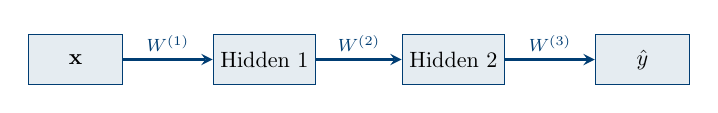
\begin{tikzpicture}[scale=0.8, transform shape]
            \tikzstyle{block} = [rectangle, draw=uibblue, fill=uibblue!10, minimum width=1.5cm, minimum height=0.8cm]
            \tikzstyle{arrow} = [thick,->,>=stealth,uibblue]
            
            \node[block] (x) at (0,0) {$\mathbf{x}$};
            \node[block] (h1) at (3,0) {Hidden 1};
            \node[block] (h2) at (6,0) {Hidden 2};
            \node[block] (y) at (9,0) {$\hat{y}$};
            
            \draw[arrow] (x) -- node[above] {\footnotesize $W^{(1)}$} (h1);
            \draw[arrow] (h1) -- node[above] {\footnotesize $W^{(2)}$} (h2);
            \draw[arrow] (h2) -- node[above] {\footnotesize $W^{(3)}$} (y);
        \end{tikzpicture}
    \end{center}
    
    \vspace{0.3cm}
    \begin{block}{Key point}
        Forward propagation calculates prediction - no learning happens here. Learning happens through backpropagation and weight updates.
    \end{block}
\end{frame}

\begin{frame}{D05: Explain backpropagation at a conceptual level}
    \textbf{Backpropagation = backward computation of error}
    
    \vspace{0.3cm}
    \textbf{Main idea:}
    \begin{enumerate}
        \item \textbf{Compute error:} Compare prediction $\hat{y}$ with ground truth $y$
        \item \textbf{Propagate backward:} How much did each weight contribute to the error?
        \item \textbf{Chain rule:} Differentiate error with respect to each weight in the network
        \item \textbf{Update weights:} Adjust to reduce error
    \end{enumerate}
    
    \vspace{0.3cm}
    \begin{alertblock}{Intuition}
        Imagine adjusting a complex machine: Backpropagation tells you which screws (weights) to turn, and in which direction, to improve the result.
    \end{alertblock}
    
    \vspace{0.3cm}
    \begin{block}{Mathematical (simplified)}
        $\frac{\partial L}{\partial w} = \frac{\partial L}{\partial \hat{y}} \cdot \frac{\partial \hat{y}}{\partial z} \cdot \frac{\partial z}{\partial w}$
        
        \small (Chain rule for derivatives propagates gradients backward through the network)
    \end{block}
\end{frame}

\begin{frame}{D06: Understand gradient descent and learning rate}
    \textbf{Gradient descent:}
    \begin{itemize}
        \item Optimization algorithm to \textbf{minimize the loss function}
        \item Follows the \textbf{negative gradient} (steepest descent)
    \end{itemize}
    
    \vspace{0.3cm}
    \textbf{Update rule:}
    \[
    w_{\text{new}} = w_{\text{old}} - \eta \cdot \frac{\partial L}{\partial w}
    \]
    
    \begin{columns}[T]
        \begin{column}{0.48\textwidth}
            \textbf{Learning rate $\eta$:}
            \begin{itemize}
                \item Determines \textbf{step size}
                \item Too large: Jumps over minimum
                \item Too small: Slow convergence
                \item Typical: 0.001--0.01
            \end{itemize}
        \end{column}
        \begin{column}{0.48\textwidth}
            \textbf{Variants:}
            \begin{itemize}
                \item \textbf{Batch GD:} All data per update
                \item \textbf{Stochastic GD:} One example at a time
                \item \textbf{Mini-batch GD:} Small batches (32--128)
                \item \textbf{Adam:} Adaptive learning rate (popular!)
            \end{itemize}
        \end{column}
    \end{columns}
    
    \vspace{0.2cm}
    \begin{block}{\footnotesize Epoch}
        \footnotesize An \textbf{epoch} = one complete pass through the entire training dataset
    \end{block}
\end{frame}

\begin{frame}{D07: Know about loss functions (cross-entropy, MSE)}
    \textbf{Loss function:}
    \begin{itemize}
        \item Measures \textbf{how wrong} the model's predictions are
        \item The goal: Minimize loss during training
    \end{itemize}
    
    \vspace{0.3cm}
    \begin{columns}[T]
        \begin{column}{0.48\textwidth}
            \textbf{MSE (Mean Squared Error):}
            \[
            L = \frac{1}{n}\sum_{i=1}^{n}(y_i - \hat{y}_i)^2
            \]
            \begin{itemize}
                \item Used for \textbf{regression}
                \item Penalizes large errors heavily
                \item Continuous output
            \end{itemize}
        \end{column}
        \begin{column}{0.48\textwidth}
            \textbf{Cross-Entropy:}
            \[
            L = -\sum_{i} y_i \log(\hat{y}_i)
            \]
            \begin{itemize}
                \item Used for \textbf{classification}
                \item Binary: $-[y\log\hat{y} + (1-y)\log(1-\hat{y})]$
                \item Measures divergence between probability distributions
            \end{itemize}
        \end{column}
    \end{columns}
    
    \vspace{0.2cm}
    \begin{block}{\footnotesize Choosing the right loss}
        \footnotesize
        \textbf{Regression:} MSE/MAE \quad \textbf{Binary:} Binary CE \quad \textbf{Multi-class:} Categorical CE
    \end{block}
\end{frame}

% =====================================================================
% SECTION: Convolutional Neural Networks
% =====================================================================
\section{Convolutional Neural Networks (CNN)}

\begin{frame}{D08: Describe a convolutional neural network (CNN)}
    \textbf{CNN = specialized for image data}
    
    \begin{itemize}
        \item Exploits \textbf{spatial structure} in images
        \item Far fewer parameters than fully connected network
        \item Translation invariant - recognizes patterns regardless of position
    \end{itemize}
    
    \vspace{0.3cm}
    \textbf{Typical CNN architecture:}
    \begin{center}
        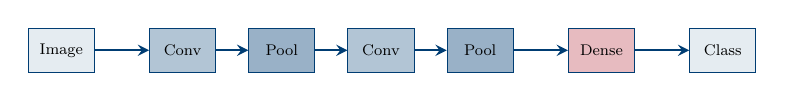
\begin{tikzpicture}[scale=0.7, transform shape]
            \tikzstyle{block} = [rectangle, draw=uibblue, fill=uibblue!10, minimum width=1.2cm, minimum height=0.8cm, font=\footnotesize]
            \tikzstyle{arrow} = [thick,->,>=stealth,uibblue]
            
            \node[block] (img) at (0,0) {Image};
            \node[block, fill=uibblue!30] (c1) at (2.2,0) {Conv};
            \node[block, fill=uibblue!40] (p1) at (4,0) {Pool};
            \node[block, fill=uibblue!30] (c2) at (5.8,0) {Conv};
            \node[block, fill=uibblue!40] (p2) at (7.6,0) {Pool};
            \node[block, fill=uibred!30] (fc) at (9.8,0) {Dense};
            \node[block] (out) at (12,0) {Class};
            
            \draw[arrow] (img) -- (c1);
            \draw[arrow] (c1) -- (p1);
            \draw[arrow] (p1) -- (c2);
            \draw[arrow] (c2) -- (p2);
            \draw[arrow] (p2) -- (fc);
            \draw[arrow] (fc) -- (out);
        \end{tikzpicture}
    \end{center}
    
    \vspace{0.3cm}
    \textbf{Hierarchical learning:}
    \begin{itemize}
        \item Early layers: Simple features (edges, textures)
        \item Later layers: Complex features (shapes, object parts)
        \item Final layer: High-level concepts (objects, categories)
    \end{itemize}
\end{frame}

\begin{frame}{D09: Explain what a convolution filter does}
    \textbf{Convolution filter (kernel):}
    \begin{itemize}
        \item Small matrix (e.g. $3 \times 3$) that \textbf{slides over the image}
        \item Calculates dot product between filter and image patch
        \item Produces a \textbf{feature map}
    \end{itemize}
    
    \vspace{0.3cm}
    \begin{columns}[T]
        \begin{column}{0.55\textwidth}
            \textbf{Example: Edge detection}
            \begin{center}
                \small
                $\begin{bmatrix} -1 & -1 & -1 \\ 0 & 0 & 0 \\ 1 & 1 & 1 \end{bmatrix}$
            \end{center}
            \begin{itemize}
                \item Detects horizontal edges
                \item Different filters $\rightarrow$ different features
                \item CNN \textbf{learns} optimal filters!
            \end{itemize}
        \end{column}
        \begin{column}{0.42\textwidth}
            \textbf{Key concepts:}
            \begin{itemize}
                \item \textbf{Stride:} How far the filter moves
                \item \textbf{Padding:} Adding pixels at the border
                \item \textbf{Channels:} RGB = 3 channels
                \item \textbf{Feature map:} Output from convolution
            \end{itemize}
        \end{column}
    \end{columns}
    
    \vspace{0.2cm}
    \begin{block}{\footnotesize Weight sharing}
        \footnotesize Same filter used across entire image $\rightarrow$ dramatically fewer parameters than a fully connected network.
    \end{block}
\end{frame}

\begin{frame}{D10: Describe pooling layers and their function}
    \textbf{Pooling = downsampling of feature maps}

    \vspace{0.2cm}
    \begin{columns}[T]
        \begin{column}{0.55\textwidth}
            \textbf{Most common type: Max pooling}
            \begin{itemize}
                \item Selects \textbf{maximum value} in each region (e.g. $2 \times 2$)
                \item Reduces spatial size by factor of 2
            \end{itemize}

            \vspace{0.2cm}
            \textbf{Advantages of pooling:}
            \begin{itemize}
                \item \textbf{Reduces computation} - fewer parameters
                \item \textbf{Translation invariance} - slight shift does not affect output
                \item \textbf{Prevents overfitting}
            \end{itemize}
        \end{column}
        \begin{column}{0.42\textwidth}
            \textbf{Example ($2 \times 2$ max pool):}
            \begin{center}
                $\begin{bmatrix} 1 & 3 \\ 2 & 4 \end{bmatrix} \rightarrow 4$

                \vspace{0.2cm}
                $\begin{bmatrix} 5 & 1 \\ 0 & 2 \end{bmatrix} \rightarrow 5$
            \end{center}

            \vspace{0.2cm}
            \begin{block}{\footnotesize Other pooling types}
                \footnotesize
                \begin{itemize}
                    \item \textbf{Average:} Mean value
                    \item \textbf{Global avg:} Feature map $\rightarrow$ one value
                \end{itemize}
            \end{block}
        \end{column}
    \end{columns}
\end{frame}

% =====================================================================
% SECTION: Regularization and Techniques
% =====================================================================
\section{Regularization and Advanced Techniques}

\begin{frame}{D11: Know about batch normalization and dropout}
    \begin{columns}[T]
        \begin{column}{0.48\textwidth}
            \textbf{Batch Normalization:}
            \begin{itemize}
                \item Normalizes activations in each mini-batch
                \item $\hat{x} = \frac{x - \mu}{\sigma}$, then scale/shift
                \item Advantages:
                \begin{itemize}
                    \item Faster training
                    \item Stabilizes learning
                    \item Allows higher learning rate
                \end{itemize}
                \item Typically placed after convolution, before activation
            \end{itemize}
        \end{column}
        \begin{column}{0.48\textwidth}
            \textbf{Dropout:}
            \begin{itemize}
                \item ``Turns off'' random neurons during training
                \item Typical dropout rate: 0.2--0.5
                \item Advantages:
                \begin{itemize}
                    \item Reduces \textbf{overfitting}
                    \item Forces network to be robust
                    \item Acts as ensemble
                \end{itemize}
                \item Used only during training!
            \end{itemize}
        \end{column}
    \end{columns}
    
    \vspace{0.5cm}
    \begin{block}{Regularization techniques}
        Both batch normalization and dropout help prevent overfitting and improve generalization.
    \end{block}
\end{frame}

\begin{frame}{D12: Understand the concept of transfer learning}
    \textbf{Transfer learning:}
    \begin{itemize}
        \item Reuse a model trained on one problem for a new problem
        \item Especially useful when you have \textbf{limited data}
    \end{itemize}
    
    \vspace{0.3cm}
    \textbf{Typical approach:}
    \begin{enumerate}
        \item Take a pretrained model (e.g. trained on ImageNet - millions of images)
        \item Freeze early layers (general features)
        \item Replace/train final layer for your specific task
        \item (Optional) Fine-tune entire model with low learning rate
    \end{enumerate}
    
    \vspace{0.3cm}
    \begin{alertblock}{\footnotesize Why does it work?}
        \footnotesize Early layers learn \textbf{general features} (edges, textures) that are useful for many tasks. Only the final layers are task-specific.
    \end{alertblock}

    \begin{block}{\footnotesize Example in medicine}
        \footnotesize Train on millions of natural images $\rightarrow$ Fine-tune on thousands of X-ray images $\rightarrow$ Better results than training from scratch!
    \end{block}
\end{frame}

\begin{frame}{D13: Know about advanced architectures (ResNet, ViT)}
    \begin{columns}[T]
        \begin{column}{0.48\textwidth}
            \textbf{ResNet (Residual Networks):}
            \begin{itemize}
                \item Introduced \textbf{skip connections}
                \item Allows gradients to flow directly
                \item Enables very deep networks (50--152+ layers)
                \item $y = F(x) + x$ (residual block)
            \end{itemize}
            
            \vspace{0.2cm}
            \textbf{Important contribution:}
            \begin{itemize}
                \item Solved the problem of degradation in deep networks
                \item Standard for medical image analysis
            \end{itemize}
        \end{column}
        \begin{column}{0.48\textwidth}
            \textbf{ViT (Vision Transformer):}
            \begin{itemize}
                \item Applies transformer architecture to images
                \item Divides image into patches (``tokens'')
                \item Uses self-attention
                \item Scales well with data and compute
            \end{itemize}
            
            \vspace{0.2cm}
            \textbf{Modern trend:}
            \begin{itemize}
                \item Outperforms CNN on large datasets
                \item Used in state-of-the-art models
            \end{itemize}
        \end{column}
    \end{columns}
    
    \vspace{0.3cm}
    \begin{block}{Other important architectures}
        \textbf{U-Net}: Segmentation (medical classic) | \textbf{EfficientNet}: Balanced scaling | \textbf{DenseNet}: Dense connections
    \end{block}
\end{frame}

% =====================================================================
% SUMMARY
% =====================================================================
\section*{Summary}

\begin{frame}{Summary: Deep Learning}
    \textbf{Fundamentals:}
    \begin{itemize}
        \item D01--D03: Neurons, MLP, activation functions
        \item D04--D07: Forward/backprop, gradient descent, loss functions
    \end{itemize}
    
    \textbf{CNN:}
    \begin{itemize}
        \item D08--D10: Architecture, convolution filters, pooling
        \item Hierarchical learning of image features
    \end{itemize}
    
    \textbf{Advanced:}
    \begin{itemize}
        \item D11: Batch normalization, dropout (regularization)
        \item D12: Transfer learning (reuse of pretrained knowledge)
        \item D13: ResNet (deep networks), ViT (transformers for images)
    \end{itemize}
    
    \vspace{0.3cm}
    \begin{block}{Lab 2 - Hands-on experience}
        Build, train and evaluate CNNs with PyTorch. Use Grad-CAM to understand model decisions.
    \end{block}
\end{frame}

\end{document}
